\documentclass[11pt]{article}
\usepackage{epsfig}    
\usepackage{float}
\usepackage[]{algorithm2e}
\usepackage{hyperref}
\setlength{\parindent}{0em}
\setlength{\parskip}{1ex}
\setlength{\AlCapSkip}{1em}
\begin{document}

\title{Estimating $\mathcal{R}_t$ from Covid-19 case counts, \\
an instruction manual for a DIY lockdown project }
\author{ Hugh Murrell and Daniel Murrell}
\maketitle

\begin{abstract}
\noindent Here we give an interpretation of
the {\it effective reproduction number}, $\mathcal{R}_t$ that arises
from the Susceptible-Infectious (SI) model 
for the spread of infectious disease. We also show that
a very simple smoothed frequentist estimator behaves 
similarly to a Bayesian posterior mean for this model.
We outline a simple  finite difference scheme for
estimating $\mathcal{R}_t$ from daily case counts.
\end{abstract}

\section{Introduction}

From the onset of the Covid-19 pandemic many articles have appeared
in the popular press claiming that $\mathcal{R}_t$ is the metric to track when trying
to ascertain the success, or lack thereof, of lockdown measures put in place
by the authorities. See \cite{groundup} for an excellent introduction to 
$\mathcal{R}_t$ and why we should be following it. 

Usually, government advisors report on the current value of $\mathcal{R}_t$
and if this value is less than one the lockdown measures are deemed to be working
but if it is greater than one then more stringent lockdown measures are recommended.
However, methods for the computation of $\mathcal{R}_t$ are seldom outlined.
The reason for this is that today's methods usually involve complicated
Bayesian inference which is deemed to lie outside the skill set of the article 
readership, see \cite{news24} for an example of an article in the South African
popular press.

An exception to the above is the work of Kevin Systrom who uses the 
Bayesian inference techniques of BettenCourt and Ribeiro \cite{bettencourt}
on regional USA case count data to obtain $\mathcal{R}_t$
values for each state and thus rank state-wide responses to the pandemic. See
\href{https://rt.live/}{https://rt.live/} for his latest rankings. 
Refreshingly, Systrom has made his methods available to the public by publishing 
his Python code with explanation as Jupyter notebooks on github \cite{systrom}.
Members of the public can download his notebooks and run them on their
own datasets.

However, to understand Systrom's Bayesian code, you need a backgound in statistics which
many readers do not have. In this article we develop a simple finite difference
algorithm for estimating $\mathcal{R}_t$ and we show that this simple algorithm
behaves similarly to the Bayesian posterior mean of Systrom's code. 

Our experiments are performed on South African datasets at national and provincial 
levels and our code is made available to the public through github.


\section{The standard SI model}
The Susceptible-Infectious (SI) model \cite{Wikipedia} is often used 
to study the spread of infectious disease by tracking the number ($S$) of people 
susceptible to the disease and the number ($I$) of people infectious with the disease.

Based on the model, the only way that a person can leave the susceptible
group is to be infected and become immediately infectious, and the only way 
that a person can leave the infectious group is to recover or die. 
It is further assumed that those who have recovered or died from the disease 
are no longer susceptible.

It is also assumed that all those who have not had the disease are 
equally susceptible and that the probability of their contracting the 
disease at time $t+1$ is proportional to the product of $S$ and $I$ at time $t$. 

These assumptions lead us to a pair of difference equations
for $S$ and $I$, where the unit of time $t$ is one day:

\begin{eqnarray}
S_{t+1} & = & S_t - \beta \frac{S_t I_t}{N} \label{eq1a} \\
I_{t+1} & = & I_t + \beta \frac{S_t I_t}{N} - \gamma I_t \label{eq1b} 
\end{eqnarray}

Here the parameter $\beta \geq 0$ controls the rate at which the susceptible
become infected and the parameter $\gamma \geq 0$ controls the rate
at which the infectious recover or die. The parameter $N$ is the size of
the {\bf initial} susceptible population and is usually assumed constant. 
The number of infected persons who are no longer infectious
is given by $N-(S_t+I_t)$.

The susceptible time series $S_t$ is a monotonically decreasing sequence
starting at $S_0 = N$ just before the outbreak of the disease whilst the infectious 
time series $I_t$ starts at $I_0 = 0$ just before the outbreak but then climbs and falls
depending on interventions but eventually dies out to zero when
the disease has run its course. 

With this model the trajectories of $S_t$ and $I_t$ are pre-determined at the outset by
the parameters, $\beta$, $\gamma$ and $N$. See Figure \ref{fig1} for an
example trajectory.

\begin{figure}[ht]
\begin{center}
  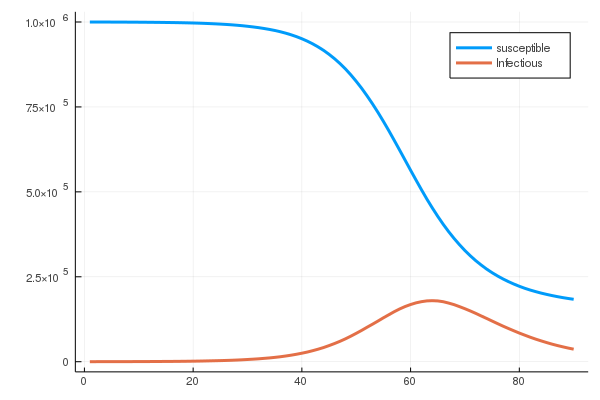
\epsfig{file=figs/fig_RtSIM.png,height=2in}
\end{center}
\caption{Susceptible and Infectious time series
for user defined parameters, $\gamma = \frac{1}{7}$, $N=10^6$ and $\beta = 2 \gamma$.
}  
\label{fig1}
\end{figure}

\section{Introducing $\mathcal{R}_t$}

To gain some {\it control} over an epidemic, authorities can enforce quarantine or
social distancing measures which may affect some of the model parameters.
The parameter $\gamma$ cannot be manipulated through such measures as it
is a property of the disease itself.
$\gamma$ is the reciprocal of the length of the infectious period of the disease 
which in the case of Covid-19 is estimated to be about one week, so $\gamma = \frac{1}{7}$.

The other two parameters, $\beta$ and $N$, can be manipulated via interventions
and it is a common practice to define a quantity called the {\it effective} reproduction number, 
$\mathcal{R}_t$ as follows:

\begin{eqnarray}
\mathcal{R}_{t} & = & \frac{\beta}{\gamma}\frac{S_t}{N} \label{eq2} 
\end{eqnarray}

and then recast the discrete SI model as:

\begin{eqnarray}
S_{t+1} & = & S_t - \gamma \mathcal{R}_t  I_t \label{eq3a} \\
I_{t+1} & = & I_t +\gamma  I_t ( \mathcal{R}_t - 1 ) \label{eq3b} 
\end{eqnarray}

Note that $ \mathcal{R}_0 = \frac{\beta}{\gamma} $
which is called the {\bf basic} reproduction number and tells us how many
persons an infected person will infect during their infectious period at the
start of an epidemic and before any interventions can be mounted.
In the case depicted in figure \ref{fig1}, the basic reproduction number is
$\mathcal{R}_0 = \frac{\beta}{\gamma} \frac{S_0}{N} = 2 $.

Note that if no interventions are put in place during the course of the epidemic 
then $\mathcal{R}_t$ will decrease monotonically as $S_t$ decreases.
The goal of interventions is to decrease $\mathcal{R}_t$ faster than
the natural decline induced by the diminishing pool of susceptible persons.
In particular it is desirable to force $\mathcal{R}_t < 1$ so that 
the pool of infectious is smaller when a person leaves the pool
than when he enters it. 

To see if an intervention is successful or not we must have some
way of estimating the current value of $\mathcal{R}_t$ from 
daily new-case counts, $C_t$, which is how most governments currently
release Covid-19 data.

\section{Estimating $\mathcal{R}_t$ from case count data}

Almost all modern attempts at estimating $\mathcal{R}_t$ implement
Bayes's rule to estimate current $\mathcal{R}_t$ from previous values
of $\mathcal{R}_t$, see for example \cite{bettencourt} for the theory 
and \cite{systrom} for a recent implementation. Here we will use a
frequentist approach and with the use of a simple smoothing filter
we will show how to estimate $\mathcal{R}_t$ directly from the data.

An {\it instantaneous} estimate for yesterday's $\mathcal{R}_t$ value can be obtained
by comparing the size of yesterday's infectious pool with the size
of today's infectious pool by rewriting equation \ref{eq3b} as 

\begin{eqnarray}
\mathcal{R}_t  & =  & 1 + \frac{1}{\gamma}  \left( \frac{ I_{t+1} - I_t} {I_t }  \right) \label{eq4} 
\end{eqnarray}

As we can estimate the current size of the infectious pool, $I(t)$,  by 
summing {\it new case counts}, $C_t$, over the preceding infectious period:

\begin{eqnarray}
I_t  & =  & \sum_{j=t-\frac{1}{\gamma}+1}^t C_t \label{eq5} 
\end{eqnarray}

Equations \ref{eq4} and \ref{eq5} provide us with an algorithm for estimating $\mathcal{R}_t$.
However are three drawbacks to this algorithm.

\begin{itemize}
\item[1)] Case reporting is very erratic due to things like testing backlogs and data collection. 
To overcome erratic reporting we will apply a smoothing filter to the time series and
assume that the real world process is not as stochastic as the actual reporting.
\item[2)] There is a natural delay, when the patient is infectious but un-diagnosed, 
between the infectious {\it onset} of the disease and the appearance of symptoms
and case {\it reporting}. 
In the literature, this problem is solved by convolving the new cases time series
with an empirical estimate of reporting delays. This procedure shifts the time series
a few days earlier and causes case counts to shrink at the end of the time series.
This shrinkage is repaired using a a technique called {\it nowcasting}. 
We will attempt to implement a simple version of onset correction 
on our Covid-19 data but even with this correction implemented we will discard
the latest $\mathcal{R}_t$ estimates for reporting purposes.
\item[3)]
The difference scheme proposed in equation \ref{eq4} is unstable when the
epidemic has been vanquished and the pool of infectious persons is near zero.
At this stage a sudden appearance of one or two new cases will send the
estimate for $\mathcal{R}_t$ sky high. The correct way to deal with this
problem is to implement Bayes' rule for updating $\mathcal{R}_t$ that requires
the calculation of {\it priors} from preceding values of $\mathcal{R}_t$ and then
selects the {\it most likely} $\mathcal{R}_t$ trajectory. We will avoid the
heavy Bayes' rule machinery by simply having an artificial cutoff that detects
when the size of the infectious pool is negligible.
\end{itemize}

\subsection{Pseudocode}

Given a new-case count time series, $\mathcal{C}_t$ , for a region an $\mathcal{R}_t$ 
time series can be computed as follows:


\begin{algorithm}[H]
\SetKwInOut{Input}{input}\SetKwInOut{Output}{output}
 \Input{$\mathcal{C}_t$ daily new-case counts}
 \Indp
truncate $\mathcal{C}_t$ by removing leading zeros\;
compute $SC_t$ as cumulative sum of $\mathcal{C}_t$\;
 {\it impute} missing values on $SC_t$ using linear interpolation\;
 reconstruct $\mathcal{C}_t$ by using first differences on $SC_t$\;
apply a moving-average filter to the $\mathcal{C}_t$ series\;
apply {\it onset estimation} to the $\mathcal{C}_t$ series\; 
apply {\it nowcasting} to $\mathcal{C}_t$\;
compute the infectious pool time series according to equation \ref{eq5}\;
compute the $\mathcal{R}_t$  time series according to equation \ref{eq4}\; 
\If{$ \frac{I_t}{max( I_t )} < \delta$}{set corresponding $\mathcal{R}_t =0$}
discard unreliable estimates due to onset correction\;
\Indm
 \Output{$\mathcal{R}_t$ effective reproduction rate estimates}
\label{alg1}
 \caption{pseudocode for constructing $\mathcal{R}_t$ }
\end{algorithm}

It remains to give further details on {\it onset estimation} and {\it nowcasting}.

\subsection{Onset estimation and nowcasting}

Onset correction translates positive case counts to the dates where they likely occurred. 
If we have the onset delay distribution, we can distribute case counts back in time 
according to that distribution. To obtain an onset distribution we need case data
that gives reporting time and estimated contraction time for each case.
In South Africa we are unable to obtain such data because the government wont
release it. So to proceed we rely on work done using USA data for the \url{rt.live} dashboard
where an empirical distribution of onset delays was obtained from US case data, 
see figure \ref{fig_empirical_onset_dist}.

\begin{figure}[H]
\begin{center}
  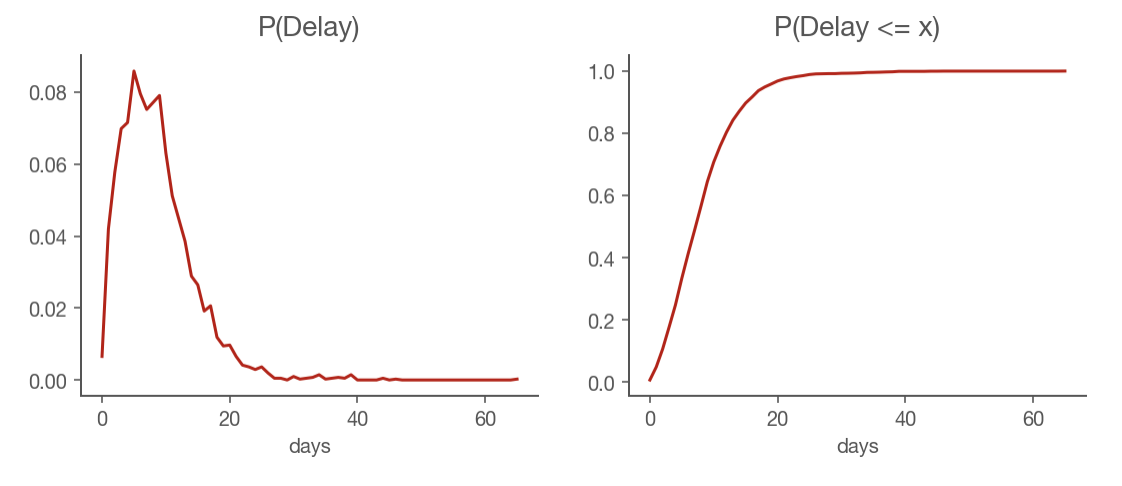
\epsfig{file=figs/fig_empirical_onset_dist.png,height=2in}
\end{center}
\caption{Empirical onset delay distribution from US case data,  see \cite{systrom} for details.}  
\label{fig_empirical_onset_dist}
\end{figure}

Although we don't have actual number for this distribution we can get some idea of its {\it shape} and
{\it scale} by studying figure \ref{fig_empirical_onset_dist} and then try and find a known statistical
distribution to do the job for us. The distribution we select is the Weibull distribution with shape 2
and scale 5, see figure \ref{fig_weibull}

\begin{figure}[H]
\begin{center}
  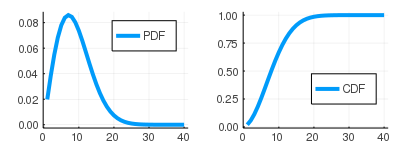
\epsfig{file=figs/fig_weibull.png,height=2in}
\end{center}
\caption{Weibull(2,5) distribution for simulating onset delay.}  
\label{fig_weibull}
\end{figure}

Now that we have an onset delay distribution to work with we can perform the onset correction.
As expained by Kevin Systrom in \cite{systrom} we accomplish this, by reversing the new-case time series, 
convolving it with the delay distribution and then reversing the series again to obtain the onset curve. 

Note that this means the data will be {\it right censored} which means there are onset cases
that have yet to be reported so it looks as if the count has gone down.
To fix the right censorship we must perform {\it nowcasting} using the CDF
of the Weibull distribution. Again in \cite{systrom}, Systrom expains how to
accomplish this:

{\it Suppose that 5 days ago, there were 100 cases onset. Over the course of the next 5 days some portion of those cases will be reported. This portion is equal to the cumulative distribution function of our delay distribution. If we know that portion is say, 60\%, then our current count of onset on that day represents 60\% of the total. This implies that the total is 166\% higher. }

We apply this correction by dividing our onset time series by the CDF of our Weilbull distribution after it has been 
augmented with a sufficient number of ones and reversed, thus removing the right censoring.
 
\section{Implementation on South African data}

We obtain the latest case counts from a github repository maintained by the Data Science for Social Impact research group
of the University of Pretoria, see \cite{dsfsi}.

The results of moving average smoothing, onset correction and nowcasting 
are depicted in figure \ref{fig_onset_now_za}.

\begin{figure}[H]
\begin{center}
  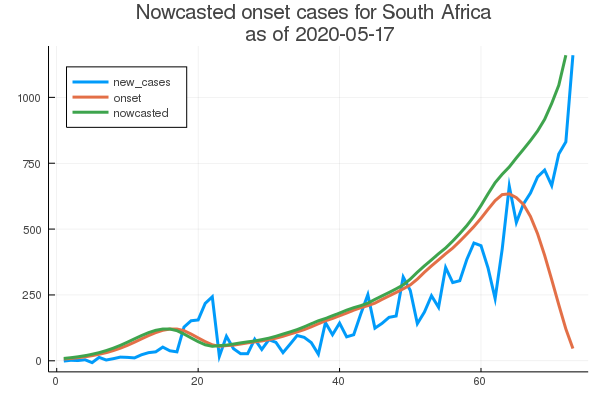
\epsfig{file=figs/fig_onset_now_ZA.png,width=4in}
\end{center}
\caption{South African case counts after onset and nowcasting correction.}  
\label{fig_onset_now_za}
\end{figure}

From the corrected new-case counts we compute the Infectious counts, $I_t$,
and then we estimate $\mathcal{R}_t$. The results, with some days discarded due
to onset correction, are shown in figure \ref{fig_rt_inf_za}.

\begin{figure}[H]
\begin{center}
  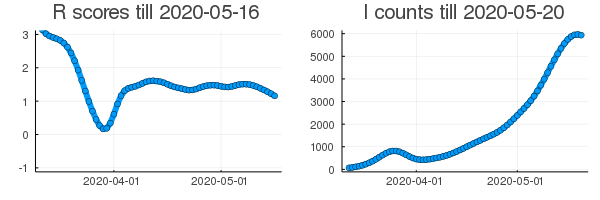
\epsfig{file=figs/fig_rt_inf_za.png,width=4in}
\end{center}
\caption{Tracking $\mathcal{R}_t$ (left) and $I_t$ (right) from South African case counts.
Note that $w$ days of $\mathcal{R}_t$ estimates have been discarded where $w$ is
the day on which the Weibull distribution peaks, in this case $w=4$.}  
\label{fig_rt_inf_za}
\end{figure}

The Julia script made available in \cite{murrell} enables the user to perform similar
analysis on South African provincial case counts. Results are shown in figure \ref{fig_rt_inf_prov}.

\begin{figure}[H]
\begin{center}
  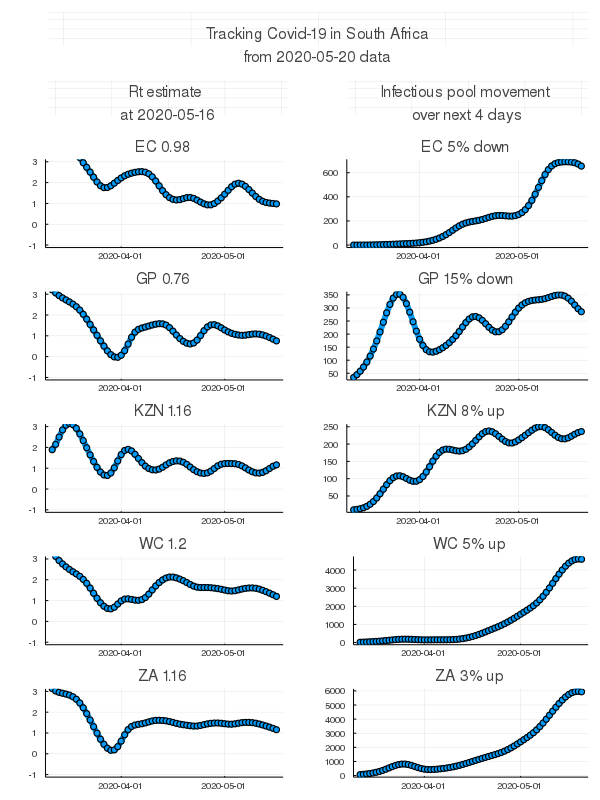
\epsfig{file=figs/fig_rt_inf_prov.png, height=6in}
\end{center}
\label{fig_rt_inf_prov}
\end{figure}

\section{Sanity check}

To provide some confidence that our simple finite difference algorithm behaves
similarly to the Bayesian posterior mean for $\mathcal{R}_t$ estimation on
South African data we  juxtapose our result with an implementation by Schalk van Heerden
for the DSFSI \cite{dsfsi} using Systrom's code, \cite{systrom}. The comparison is shown in figure \ref{fig_heerden}.

\begin{figure}[H]
\begin{center}
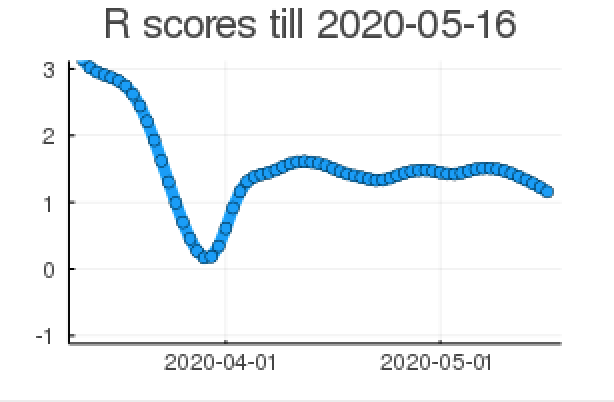
\epsfig{file=figs/fig_rt_za.png,width=3in}
  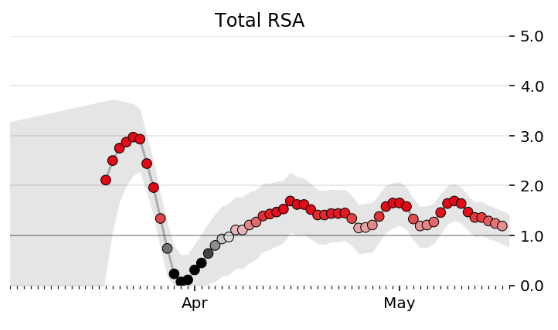
\epsfig{file=figs/fig_heerden.png,width=3in}
\end{center}
\caption{Comparing South African $\mathcal{R}_t$ trajectories, a frequentist approach (top)
and a Bayesian approach (bottom).}
\label{fig_heerden}
\end{figure}

\section{Conclusions}
The results of our simple frequentist implementation look fairly reasonable.
The technique affords the layman the opportunity to analyse his own data
and tweak model parameters as he sees fit.
thso they might be
used to decide on a strategy for curtailing an epidemic through
quarantines, lockdowns and social distancing.  
Many enhancements to the model can be made.  For a discussion 
of some of these, see \cite{systrom}.  

\section{Acknowledgements}

First and foremost, the authors thank Kevin Systrom for making his code and methods
available via github \cite{systrom}.

We also like thank {\it MediaHack} for displaying our $\mathcal{R}_t$ charts
on their South African Covid-19 dashboard and making this document available for 
public consumption via their website, \cite{mediahack}.

We also thank Benjamin Murrell for enlightening us as to the intricacies of Bayesian techniques.

\begin{thebibliography}{99}

\bibitem{bettencourt}Bettencourt MA and Ribeiro RM, {\em Real Time Bayesian Estimation of the Epidemic Potential of Emerging Infectious Diseases}, Plos One, Volume 3, Issue 5, May 2008.

\bibitem{Wikipedia} {\em Compartmental models in epidemiology},
\href{http://en.wikipedia.org/wiki/Compartmental_models_in_epidemiology}{wikipedia}

\bibitem{systrom} Kevin Systrom, 
\href{https://github.com/k-sys/covid-19/blob/master/Realtime%20Rt%20mcmc.ipynb}{github repository}

\bibitem{groundup} Max Price, Covid-19: {\em Making sense of R}, 
\href{https://www.groundup.org.za/article/covid-19-making-sense-of-r}{GroundUp article}

\bibitem{news24} Sarah Evans, {\em Lockdown and other interventions potentially saved 20 000 lives},News 24, \href{https://www.news24.com/SouthAfrica/News/lockdown-and-other-interventions-potentially-saved-20-000-lives-top-scientist-20200513}{news24 article}

\bibitem{dsfsi} Data Science for Social Impact research group, University of Pretoria, \href{https://raw.githubusercontent.com/dsfsi/covid19za/master/data/covid19za_provincial_cumulative_timeline_confirmed.csv} {github repository}
 
\bibitem{mediahack}Media Hack Collective, {\em Coronavirus in South Africa},
\href{https://mediahack.co.za/datastories/coronavirus/dashboard/}{Dashboard}.

\bibitem{murrell}Hugh Murrell, {\em SIR models for Covid-19 data},
\href{https://hughmurrell.github.io/CoVmodel/index.html}{hughmurrell.github.io/CoVmodel/index.html}.

\end{thebibliography}
\end{document}


